\section{Grundlegende Architektur}\label{sec:architecture}

\begin{wrapfigure}{r}{0.5\columnwidth}
    \centering
    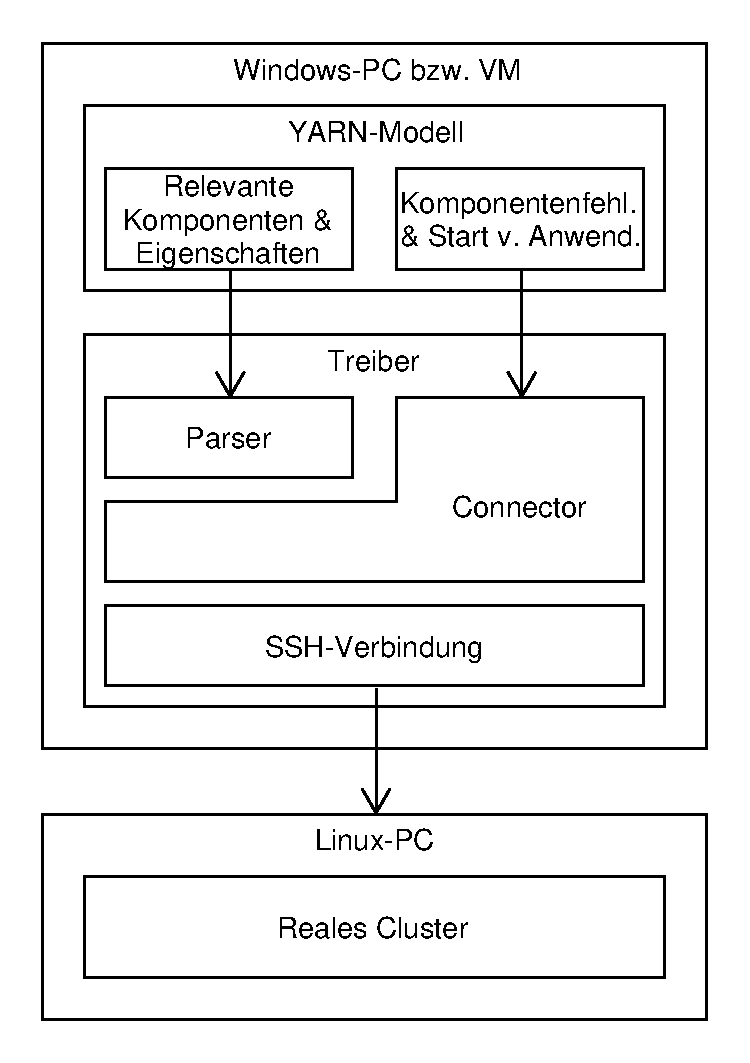
\includegraphics[width=0.5\columnwidth]{./images/modelArchitecture.pdf}
    \caption{Grundlegende Architektur des Gesamtmodells}
    \label{fig:modelArchitecture}
\end{wrapfigure}

Die grundlegende Architektur des gesamten Aufbaus besteht aus den drei rechts abgebildeten Schichten. Die oberste Schicht bildet das \sS-Modell von Hadoop YARN, welches die relevanten YARN-Komponenten und Komponentenfehler abbildet. Das reale Pendant dazu bildet das reale Hadoop-Cluster auf einem eigenen PC als unterste Schicht. Die Verbindung zwischen Modell und realem Cluster bildet der Treiber als eigenständige Schicht. Der Treiber besteht aus folgenden Komponenten:

\begin{description}[noitemsep]
    \item [Parser] Verarbeitet die Monitoring-Ausgaben vom realen Cluster und konvertiert diese für die Nutzung im Modell.
    \item [Connector] Abstrahiert die SSH-Verbindung
    \item [SSH-Verbindung] Eigentliche Verbindung zum PC mit dem realen Cluster
\end{description}

Auf den Treiber bzw. das reale System wird meist über den Parser zugegriffen. Lediglich zum Starten von Anwendungen, zum Aktivieren bzw. Deaktivieren von Komponentenfehlern u.\,Ä. auf dem realen Cluster wird direkt auf den Connector zugegriffen.